\runningheader{SAT Mathematics}{Drill Set 2}{Page \thepage\ of \numpages}

\begingradingrange{sat-drill-02}
\subsection*{SAT Drill 2}

\question[1]
\phantom{\space}\\

\begin{center}
  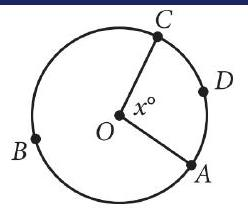
\includegraphics[width=0.70\linewidth]{images/2025_06_15_44388a8c3a9d04fd81aag-01}
\end{center}
The circle above has center $O$, the length of arc $\overline{ADC}$ is $5\pi$, and $x=100$. What is the length of arc $\overline{ABC}$?
\begin{choices}
  \choice $9\pi$
  \CorrectChoice $13\pi$
  \choice $18\pi$
  \choice $\frac{13}{2}\pi$
\end{choices}

\question[1]
The graph of $x^{2}+x+y^{2}+y=\frac{199}{2}$ in the $xy$-plane is a circle. What is the length of the circle's radius?
\begin{solutionorbox}
Completing the square gives $\bigl(x+\tfrac12\bigr)^2+\bigl(y+\tfrac12\bigr)^2=100$, so $r=10$.
\end{solutionorbox}

\question[1]
The equation above defines a circle in the $xy$-plane. What are the coordinates of the center of the circle?
\begin{choices}
  \choice $(-20,-16)$
  \CorrectChoice $\left(-\tfrac12,-\tfrac12\right)$
  \choice $(10,8)$
  \choice $(20,16)$
\end{choices}



\question[1]
\phantom{\space}\\

\begin{center}
  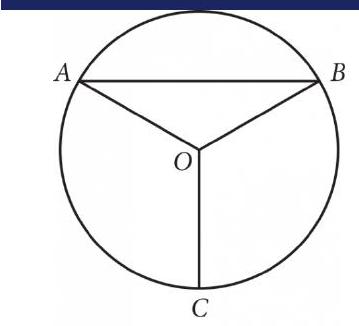
\includegraphics[width=0.70\linewidth]{images/2025_06_15_44388a8c3a9d04fd81aag-04}
\end{center}
Point $O$ is the center of the circle above, and the measure of $\angle OAB$ is $30^{\circ}$. If the length of $\overline{OC}$ is 18, what is the length of arc $\overline{AB}$?
\begin{choices}
  \choice $9\pi$
  \CorrectChoice $12\pi$
  \choice $15\pi$
  \choice $18\pi$
\end{choices}

\question[1]
A circle in the $xy$-plane has a diameter with endpoints $(2,4)$ and $(2,14)$. An equation of this circle is $(x-2)^{2}+(y-9)^{2}=r^{2}$, where $r$ is a positive constant. What is the value of $r$?
\begin{solutionorbox}
The diameter has length $|14-4|=10$, so $r=5$.
\end{solutionorbox}


\newpage



\question[1]
\phantom{\space}\\

\begin{center}
  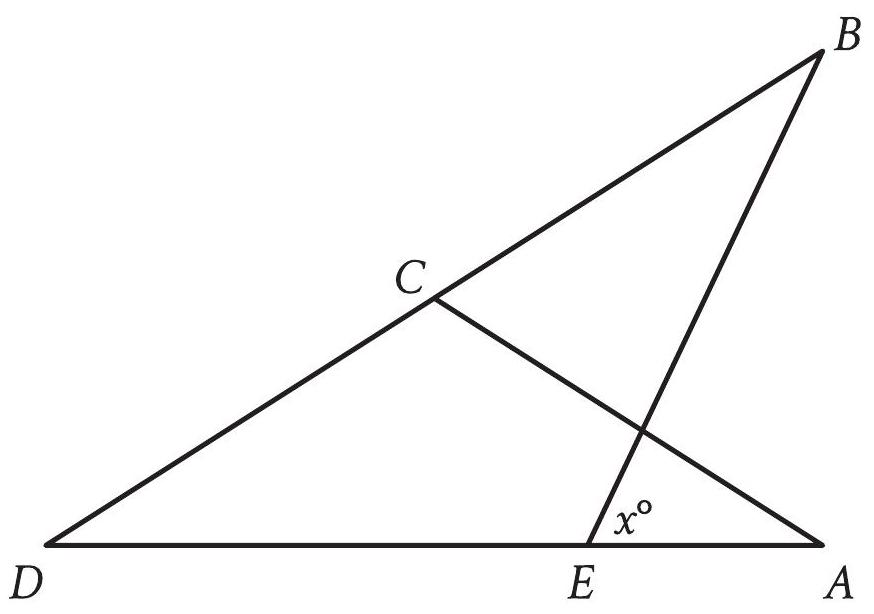
\includegraphics[width=0.70\linewidth]{images/2025_06_15_d0312806c0eedc278ae1g-01}
\end{center}
In the figure, $AC=CD$. The measure of angle $EBC$ is $45^{\circ}$, and the measure of angle $ACD$ is $104^{\circ}$. What is the value of $x$?
\begin{solutionorbox}
Triangle $ACD$ is isosceles with $\angle ACD=104^{\circ}$, so $\angle CDA=\angle CAD=38^{\circ}$. In triangle $BDE$, $\angle DEB=97^{\circ}$, which is supplementary to $x$, so $x=83$.
\end{solutionorbox}


\question[1]
\phantom{\space}\\

\begin{center}
  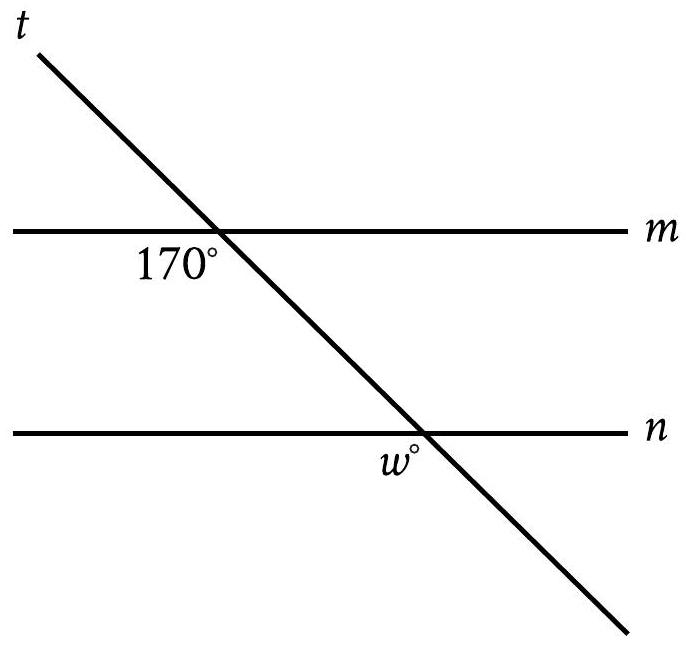
\includegraphics[width=0.70\linewidth]{images/2025_06_15_d0312806c0eedc278ae1g-04}
\end{center}
In the figure, line $m$ is parallel to line $n$. What is the value of $w$?
\begin{choices}
  \choice 17
  \choice 30
  \choice 70
  \CorrectChoice 170
\end{choices}




\newpage





\question[1]
\phantom{\space}\\

\begin{center}
  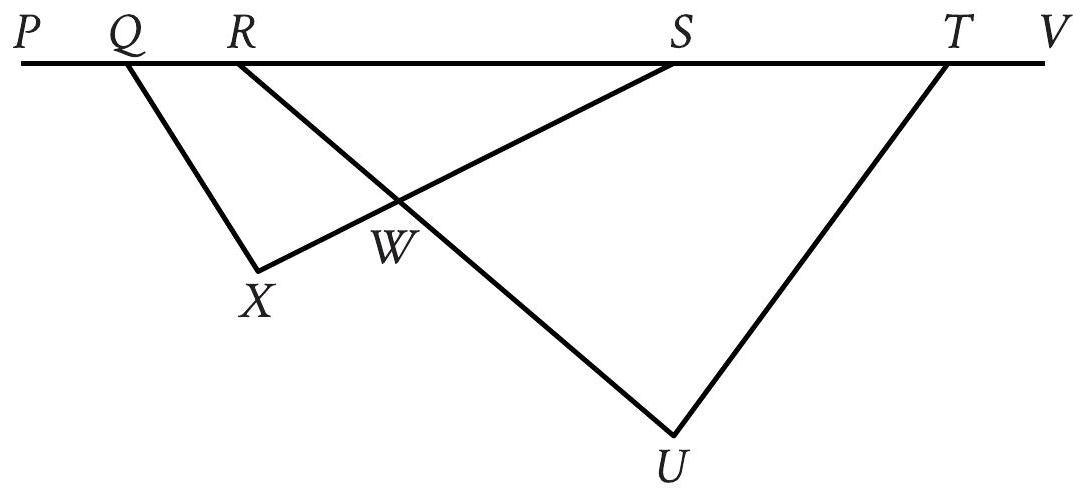
\includegraphics[width=0.70\linewidth]{images/2025_06_15_d0312806c0eedc278ae1g-02}
\end{center}
In the figure shown, points $Q$, $R$, $S$, and $T$ lie on line segment $PV$, and line segment $RU$ intersects line segment $SX$ at point $W$. The measure of $\angle SQX$ is $48^{\circ}$, the measure of $\angle SXQ$ is $86^{\circ}$, the measure of $\angle SWU$ is $85^{\circ}$, and the measure of $\angle VTU$ is $162^{\circ}$. What is the measure, in degrees, of $\angle TUR$?
\begin{solutionorbox}
In triangle $SQX$, the angle at $S$ is $180^{\circ}-48^{\circ}-86^{\circ}=46^{\circ}$. Since $\angle SWU=85^{\circ}$, its supplement along line $RU$ is $95^{\circ}$, so in triangle $RSW$ the angle at $R$ is $180^{\circ}-46^{\circ}-95^{\circ}=39^{\circ}$. Since $\angle VTU=162^{\circ}$, its supplement $\angle STU=18^{\circ}$. Thus $\angle TUR=180^{\circ}-39^{\circ}-18^{\circ}=123$.
\end{solutionorbox}


\question[1]
Intersecting lines $r$, $s$, and $t$ are shown below.
\phantom{\space}\\

\begin{center}
  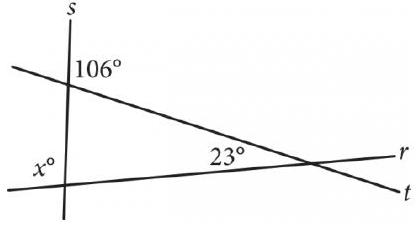
\includegraphics[width=0.70\linewidth]{images/2025_06_15_d0312806c0eedc278ae1g-03}
\end{center}
What is the value of $x$?
\begin{solutionorbox}
Angle $x$ is an exterior angle for the triangle formed by lines $r$, $s$, and $t$; with interior angles $23^{\circ}$ and $180^{\circ}-106^{\circ}=74^{\circ}$, we get $x=23+74=97$.
\end{solutionorbox}




\newpage




\question[1]
\phantom{\space}\\

\begin{center}
  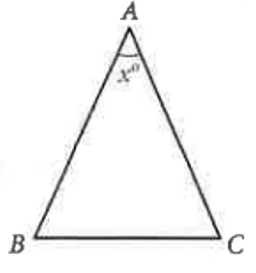
\includegraphics[width=0.40\linewidth]{images/cus07}
\end{center}
In the given triangle, $AB=AC$ and $\angle ABC$ has a measure of $67^{\circ}$. What is the value of $x$?
\begin{choices}
  \choice 36
  \CorrectChoice 46
  \choice 58
  \choice 70
\end{choices}

\question[1]
\phantom{\space}\\

\begin{center}
  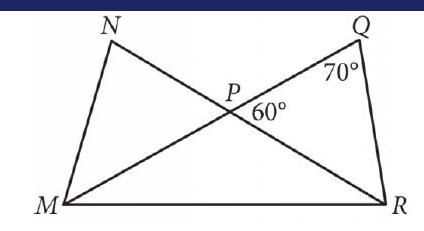
\includegraphics[width=0.70\linewidth]{images/2025_06_15_d0312806c0eedc278ae1g-06}
\end{center}
In the figure above, $\overline{MQ}$ and $\overline{NR}$ intersect at point $P$, $NP=QP$, and $MP=PR$. What is the measure, in degrees, of $\angle QMR$? (Disregard the degree symbol when gridding your answer.)
\begin{solutionorbox}
As shown in the figure, the vertical angles at $P$ measure $60^{\circ}$ and $120^{\circ}$; isosceles triangle $MPR$ has vertex angle $120^{\circ}$, so the base angles $\angle QMR$ and $\angle MRN$ are each $30$.
\end{solutionorbox}




\newpage




\question[1]
\phantom{\space}\\

\begin{center}
  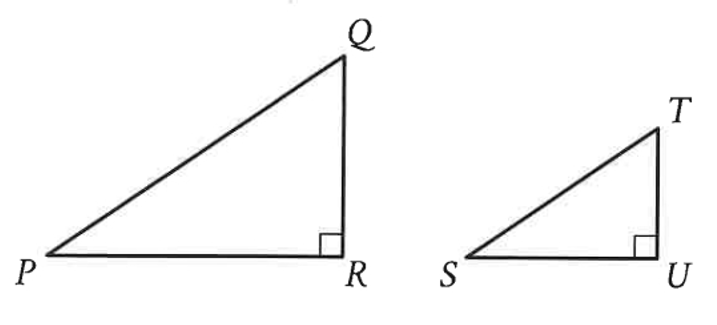
\includegraphics[width=0.70\linewidth]{images/cus08}
\end{center}
Right triangles $PQR$ and $STU$ are similar, where $P$ corresponds to $S$. If the measure of angle $Q$ is $18^{\circ}$, what is the measure of angle $S$?
\begin{choices}
  \choice $18^{\circ}$
  \CorrectChoice $72^{\circ}$
  \choice $82^{\circ}$
  \choice $162^{\circ}$
\end{choices}

\question[1]
\phantom{\space}\\

\begin{center}
  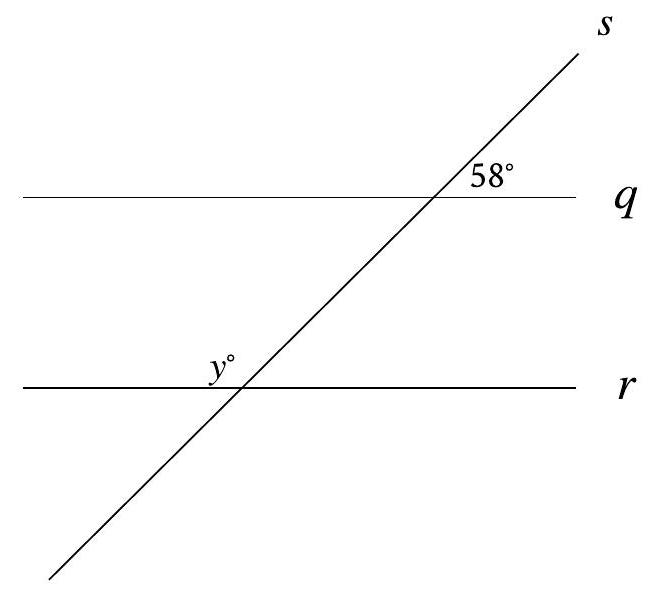
\includegraphics[width=0.70\linewidth]{images/2025_06_15_d0312806c0eedc278ae1g-08}
\end{center}
In the figure, line $q$ is parallel to line $r$, and both lines are intersected by line $s$. If $y=2x+8$, what is the value of $x$?
\begin{solutionorbox}
Same-side interior angles between parallels $q$ and $r$ are supplementary: $(2x+8)+58=180$, hence $2x=114$ and $x=57$.
\end{solutionorbox}




\newpage





\question[1]
\phantom{\space}\\
\begin{center}
  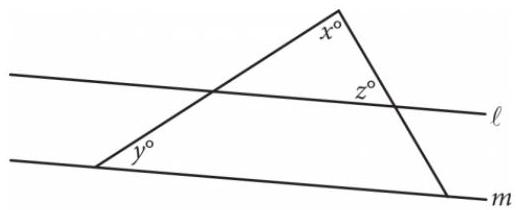
\includegraphics[width=0.70\linewidth]{images/2025_06_15_d0312806c0eedc278ae1g-09}
\end{center}
In the figure above, lines $\ell$ and $m$ are parallel, $y=20$, and $z=60$. What is the value of $x$?
\begin{choices}
  \choice 120
  \CorrectChoice 100
  \choice 90
  \choice 80
\end{choices}

\question[1]
\phantom{\space}\\

\begin{center}
  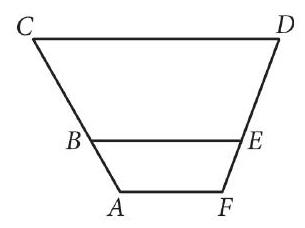
\includegraphics[width=0.70\linewidth]{images/2025_06_15_d0312806c0eedc278ae1g-10}
\end{center}
In the figure above, $\overline{AF}$, $\overline{BE}$, and $\overline{CD}$ are parallel. Points $B$ and $E$ lie on $\overline{AC}$ and $\overline{FD}$, respectively. If $AB=9$, $BC=18.5$, and $FE=8.5$, what is the length of $\overline{ED}$, to the nearest tenth?
\begin{choices}
  \choice 16.8
  \CorrectChoice 17.5
  \choice 18.4
  \choice 19.6
\end{choices}





\newpage







\question[1]
Triangle $FGH$ is similar to triangle $JKL$, where angle $F$ corresponds to angle $J$ and angles $G$ and $K$ are right angles. If $\sin(F)=\frac{308}{317}$, what is the value of $\sin(J)$?
\begin{choices}
  \choice $\frac{75}{317}$
  \CorrectChoice $\frac{308}{317}$
  \choice $\frac{317}{308}$
  \choice $\frac{317}{75}$
\end{choices}

\question[1]
In right triangle $RST$, the sum of the measures of angle $R$ and angle $S$ is 90 degrees. The value of $\sin(R)$ is $\frac{\sqrt{15}}{4}$. What is the value of $\cos(S)$?
\begin{choices}
  \choice $\frac{\sqrt{15}}{15}$
  \CorrectChoice $\frac{\sqrt{15}}{4}$
  \choice $\frac{4\sqrt{15}}{15}$
  \choice $\sqrt{15}$
\end{choices}


\question[1]
\phantom{\space}\\

\begin{center}
  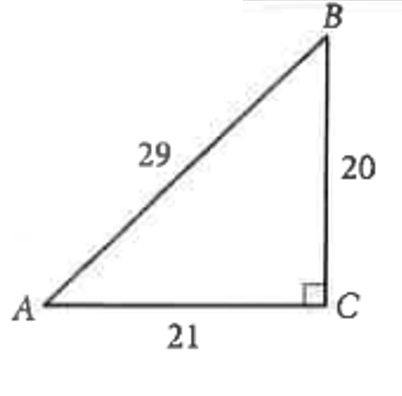
\includegraphics[width=0.60\linewidth]{images/cus09}
\end{center}
In the figure above, what is the value of $\tan(A)$?
\begin{choices}
  \choice $\frac{20}{29}$
  \choice $\frac{21}{29}$
  \CorrectChoice $\frac{20}{21}$
  \choice $\frac{21}{20}$
\end{choices}




\newpage




\question[1]
\phantom{\space}\\

\begin{center}
  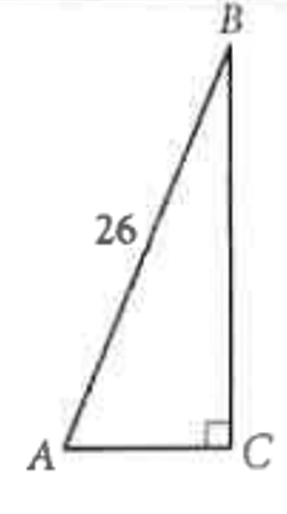
\includegraphics[width=0.40\linewidth]{images/cus10}
\end{center}
Triangle $ABC$ above is a right triangle, and $\sin(B)=\frac{5}{13}$. What is the length of side $\overline{BC}$?
\begin{solutionorbox}
With the right angle at $C$, $\sin(B)=\dfrac{AC}{AB}=\dfrac{5}{13}$ gives $AC=5$ and $BC=\sqrt{13^{2}-5^{2}}=12$.
\end{solutionorbox}



\question[1]
\phantom{\space}\\

\begin{center}
  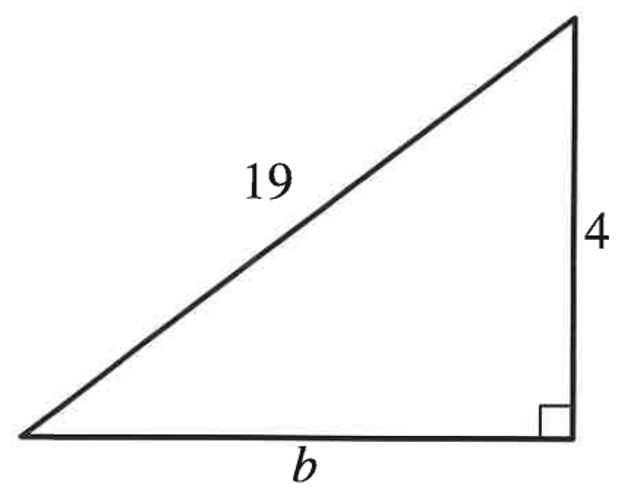
\includegraphics[width=0.70\linewidth]{images/cus11}
\end{center}
Which equation shows the relationship between the side lengths of the given triangle?
\begin{choices}
  \choice $4b=19$
  \choice $4+b=19$
  \CorrectChoice $4^{2}+b^{2}=19^{2}$
  \choice $4^{2}-b^{2}=19^{2}$
\end{choices}

\endgradingrange{sat-drill-02} 